\documentclass[addpoints,12pt]{exam}
%\documentclass[12pt]{article}
\usepackage[letterpaper, margin=0.75in]{geometry}
\usepackage{graphicx}
\usepackage{enumitem}
\usepackage{booktabs}
\usepackage{tabularx}
\usepackage{color}
\usepackage{wrapfig}

\begin{document}
\footer{}{Page \thepage\ of \numpages}{}

\begin{center}

\includegraphics[width=10cm]{../images/logo.png}
\end{center}

\begin{center}
\noindent{\LARGE Conceptual Physics \\ Second Test\\ Solutions \\}
\end{center}

 
\clearpage

\begin{flushright}
Score: \hspace{0.2in} / \numpoints ~ points
\end{flushright}

\begin{questions}
\question \textbf{Drawing Field Lines:} Four point charges are arranged in 2 different configurations, resulting in different electric fields. Assume that the size of all charges are the same, and consider only the fact that some are positive and others are negative.

\begin{parts}

\part[2] Draw the electric field lines around the following:
\vspace{0.25in}
\begin{center}
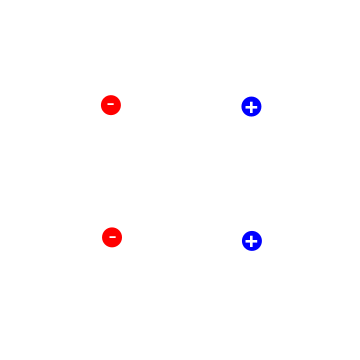
\includegraphics[width=3in]{../images/4chargesA.png}
\end{center}
\vspace{0.25in}

\part[2] Draw the electric field lines around the following:
\vspace{0.25in}
\begin{center}
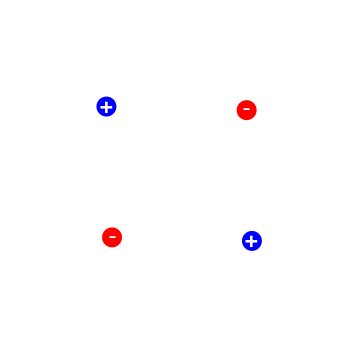
\includegraphics[width=3in]{../images/4chargesB.png}
\end{center}
\vspace{0.25in}
\end{parts}

\clearpage
\question \textbf{Lightening on a Train:} A train is moving past a platform at a velocity $v$. Lightning bolts strike the front and back of the train, scorching both the train and the platform, as the train passes the platform. An observer at rest on the platform says the strikes were simultaneous. (Hint: For this problem, it may be easiest to draw diagrams on the extra scratch paper.)
\begin{center}
	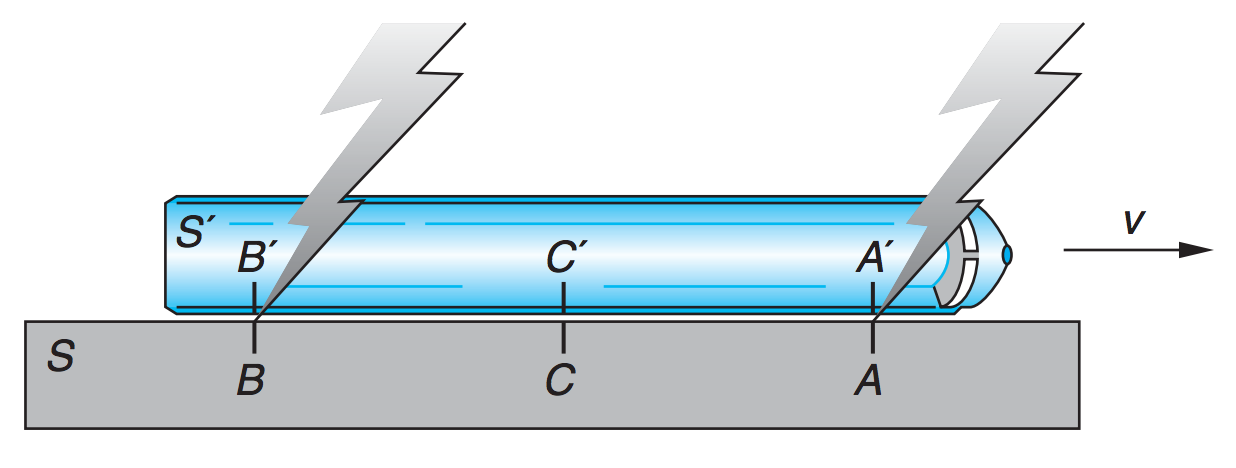
\includegraphics[width=0.7\textwidth]{../images/test2_lightning.png}
	\end{center}
	
	\begin{parts}
		\part[2] A person on the platform says that the distance between \textit{scorched marks on the platform} is \textit{D}. To a person on the train, the distance between \textit{scorch marks on the platform} is:
		\begin{choices}
			\choice Longer than \textit{D}.
			\choice Shorter than \textit{D}.
			\choice Exactly \textit{D}.
			\choice Cannot say, we need more information.
		\end{choices}
		\begin{TheSolution}
			\textbf{B.} To a person on the train, they are stationary and the platform is moving. The platform is therefore length-contracted, and so they would see it as less than \textit{D}.
		\end{TheSolution}
		\part[2] A person in the train measures the length of the train to be \textit{L}. To a person on the platform, is the train:
		\begin{choices}
			\choice Longer than \textit{L}.
			\choice Shorter than \textit{L}.
			\choice Exactly \textit{L}.
			\choice Cannot say, we need more information.
		\end{choices}
		\begin{TheSolution}
			\textbf{B.} To a person on the platform, they are stationary and the train is moving. The train is therefore length-contracted, and so they would see it as less than \textit{L}.
		\end{TheSolution}
		\part[2] A person on the platform say that the distance between the \textit{scorch marks on the train} is also \textit{D} (since they see the strikes as happening at the same time). To a person on the train, the distance between \textit{scorch marks on the train} is:
		\begin{choices}
			\choice Longer than \textit{D}.
			\choice Shorter than \textit{D}.
			\choice Exactly \textit{D}.
			\choice Cannot say, we need more information.
		\end{choices}
		\begin{TheSolution}
			\textbf{A.} To a person on the platform, the train is length contracted and so appears shorter than it does to a person on the train: this is true for all measured lengths along the train. They would therefore see the distance between train scorch marks as shorter than a person on the train. Conversely a person on the train sees the train scorch marks as longer than would a person on the platform.
		\end{TheSolution}
		\part[2] A person on the platform says the two strikes were simultaneous. What would a person on the train say?
		\begin{choices}
			\choice They would agree, the strikes happened simultaneously.
			\choice They would disagree, and say that the strike at \textit{A'} occurred before the strike at \textit{B'}
			\choice They would disagree, and say that the strike at \textit{B'} occurred before the strike at \textit{A'}
			\choice Cannot say, it is impossible for the person on the train to determine the order the strikes occurred.
		\end{choices}
		\begin{TheSolution}
			\textbf{B.} To a person on the train, the distance between scorch marks on the platform is less than \textit{D}, whereas the distance between scorch marks on the train is greater than \textit{D}. In order for this to occur, lighting would need to strike \textit{A'} before \textit{B'.}
		\end{TheSolution}
	\end{parts}

\question \textbf{Electron Energies:} Three electrons have different energies. Using the ideas of wave/particle duality, we can represent the electrons as waves. The following images shows what their wavelength looks like:

\begin{center}
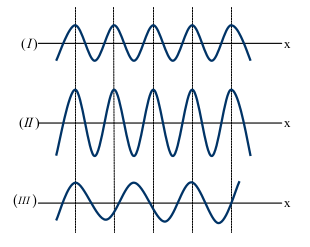
\includegraphics[width=4in]{../images/deBroglie.png}
\end{center}

The following questions will ask about how their energies, $E_I$, $E_{II}$, and $E_{III}$, relate.

\begin{parts}
	\part[2] How do $E_I$ and $E_{II}$ compare?
		\begin{choices}
			\choice $E_{I} = E_{II}$
			\choice $E_{I} > E_{II}$
			\choice $E_{I} < E_{II}$
		\end{choices}
		\begin{TheSolution}
		\textbf{A.} Since the wavelength of the two are the same, the energies need to be the same.
		\end{TheSolution}
		\part[2] How do $E_I$ and $E_{III}$ compare?
		\begin{choices}
			\choice $E_{I} = E_{III}$
			\choice $E_{I} > E_{III}$
			\choice $E_{I} < E_{III}$
		\end{choices}
		\begin{TheSolution}
			\textbf{B.} Since the wavelength of I is smaller than the wavelength at II, it must have a greater energy.
		\end{TheSolution}
	\part[2] How do $E_{II}$ and $E_{III}$ compare?
		\begin{choices}
			\choice $E_{II} = E_{III}$
			\choice $E_{II} > E_{III}$
			\choice $E_{II} < E_{III}$
		\end{choices}
		\begin{TheSolution}
			\textbf{B.} Since the wavelength of II is smaller than the wavelength of III, it must have the greater energy.
		\end{TheSolution}
\end{parts}

	\question \textbf{Balls in a Jar:} You have a jar with 6 red balls and 4 green balls.
\begin{parts}
\part[2] What is the probability of randomly drawing a red ball? What is the probability of randomly drawing a green ball?
\begin{TheSolution}
$P(\texttt{red}) = 6/10 = 0.6$, $P(\texttt{green}) = 4/10 = 0.4$. 
\end{TheSolution}
\part[2] You randomly draw one ball, put it back, and draw a ball again. What is the probability of drawing a red and a green ball, in no particular order?
\begin{TheSolution}
There are two ways to do this: draw a red ball then a green ball, or draw a green ball then a red ball. $P(\texttt{red then green}) = 0.6\cdot 0.4 = 0.24$, $P(\texttt{green then red}) = 0.4\cdot 0.6 = 0.24$, so the probability of one or the other happening is 0.24 + 0.24 = 0.48.
\end{TheSolution}
\part[2] You randomly draw one ball then draw another without putting back the first. What is the probability of drawing two red balls?
\begin{TheSolution}
On the first draw your probability of drawing red is 0.6. After drawing one red ball without replacement, your probability of drawing another red ball is 5/9, so your probability of drawing two red balls this way is $\frac{6}{10}\cdot\frac{5}{9} = 1/3$.
\end{TheSolution}
\part[2] You randomly draw one ball then draw another without putting back the first. What is the probability of drawing a red and a green ball, in no particular order?
\begin{TheSolution}
There are two ways of doing this. One is to draw a red ball then a green ball; in this case, after drawing a red ball, your probability of drawing a green ball is 4/9, so $P(\texttt{red then green, no replacement}) = \frac{6}{10}\cdot\frac{4}{9} = \frac{24}{90} = \frac{4}{15}$. The other way is to draw a green ball then a red ball; in this case, after drawing a green ball, your probability of drawing a red ball is 6/9, so $P(\texttt{green then red, no replacement}) = \frac{4}{10}\cdot\frac{6}{9} = \frac{4}{15}$. The probability of either sequence of events happening is then 4/15 + 4/15 = 8/15.
\end{TheSolution}
\end{parts}

\question \textbf{Photoelectric Effect:} Consider the following experimental setups. Light of a given wavelength is incident on one of two  metal plates sealed inside a vacuum tube. The two plates are connected in circuit to an ammeter, a device that measures electric current. The metal plates have been thoroughly cleaned so that when blue light ($\lambda = 450$~nm) is incident on the lower plate, electrons are ejected.
\begin{parts}
\part[2] There are two lightbulbs, which emit light at 300 nm and 400 nm. These wavelengths are shorter than blue light. Is the energy of the photons emitted by these two lightbulbs:
	\begin{choices}
		\choice The same as the energy contained in blue light (with wavelength 450 nm).
		\choice Greater than the energy contained in a blue light (with wavelength 450 nm).
		\choice Less than the energy contained in a blue light (with wavelength 450 nm).
	\end{choices}
	\begin{TheSolution}
	\textbf{B.} Since the wavelengths are both smaller than blue light, they have higher energy.
	\end{TheSolution}
\part[2] In the following two setups, light of 300 nm and 400 nm wavelength (ultraviolet light) is incident on the lower plates. The number of photons landing on the metal plate per second is the same in both setups (they have the same intensity). Compare the number and energy of emitted electrons in the two setups.
\begin{center}
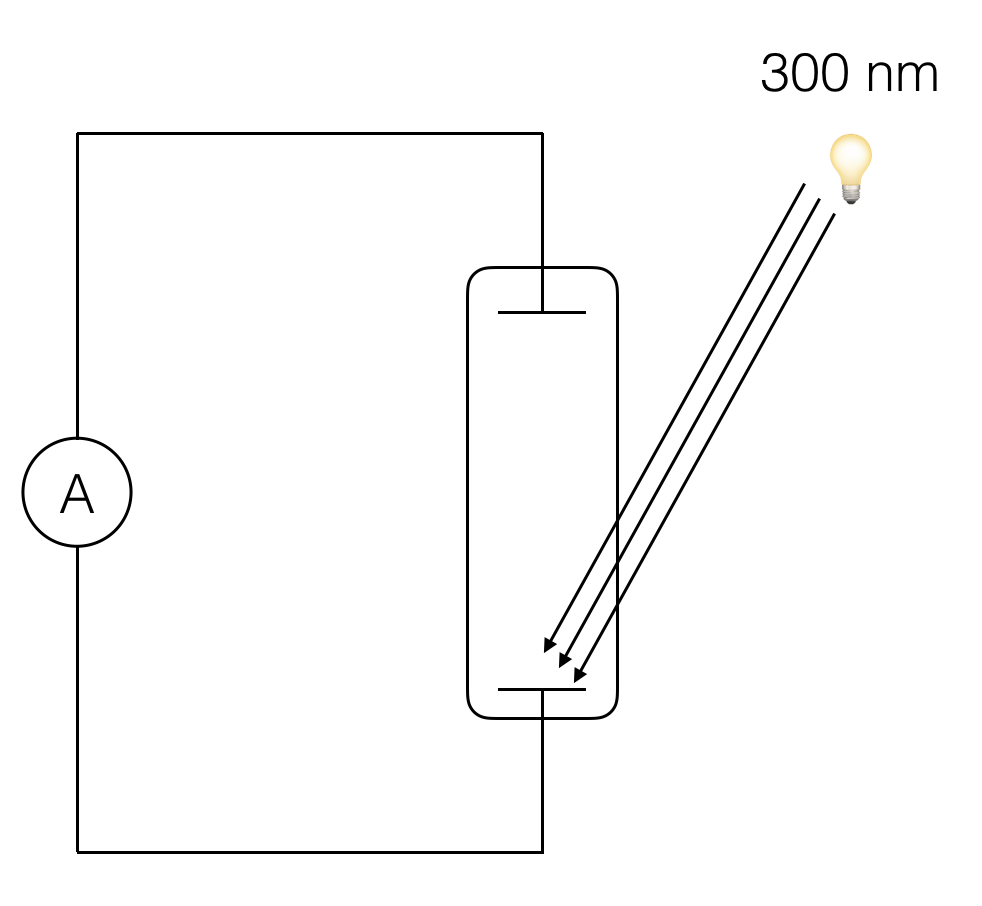
\includegraphics[width=0.45\textwidth]{../images/test2_300nm.png} 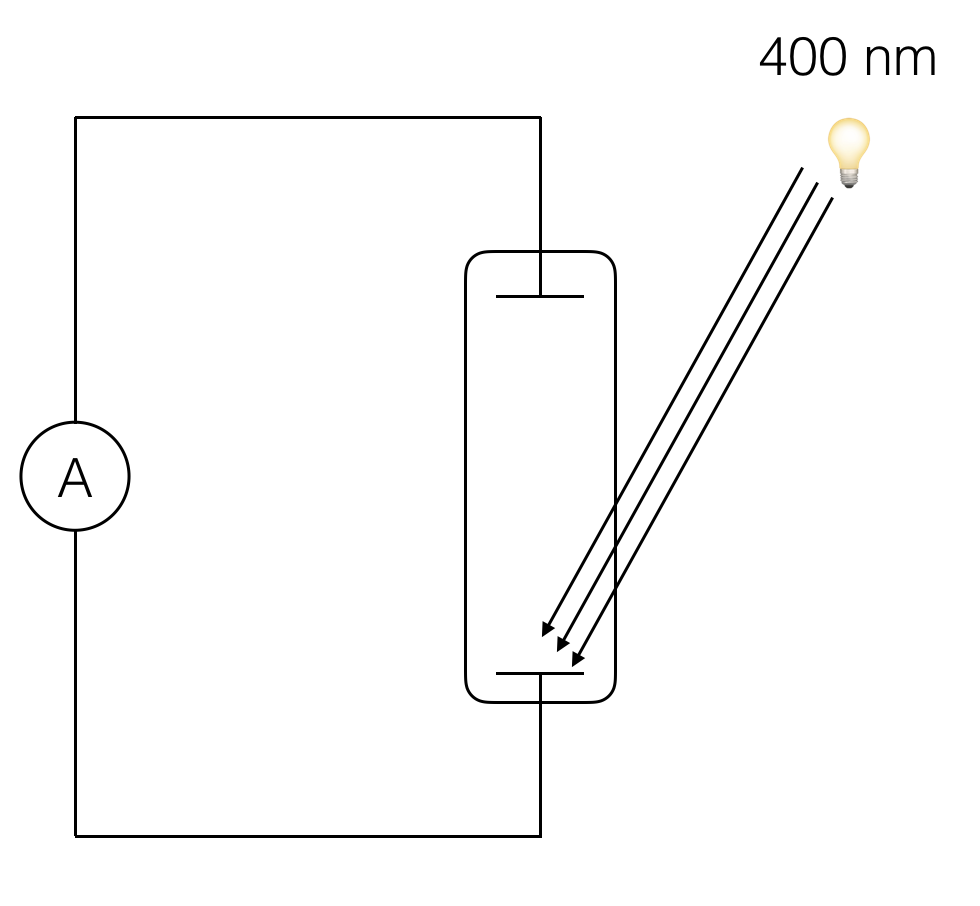
\includegraphics[width=0.45\textwidth]{../images/test2_400nm.png}
\end{center}
	\begin{choices}
		\choice The two setups emit the same number of electrons, however the setup on the left emits electrons with greater energies.
		\choice The two setups emit the same number of electron, however the setup on the right emits electrons with greater energies.
		\choice The two setups emit electrons at the same energies, however the setup on the left emits more.
		\choice The two setups emit electrons at the same energies, however the setup on the right emits more.
		\choice The two setups emit the same number of electrons and at the same energies.
	\end{choices}
	\begin{TheSolution}
		\textbf{A.} Since the intensities are the same, the number of emitted electrons is the same in both setups. However, since light on the left has a shorter wavelength than the light on the right, it has more energy and thus transfers more energy to the electrons.
	\end{TheSolution}

\part[2] In the following two setups, light of 300 nm wavelength (ultraviolet light) is incident on the lower plates. There are three times as many photons landing on the metal plate per second in the setup on the left (the left light has a greater intensity). Compare the number and energy of emitted electrons in the two setups.
\begin{center}
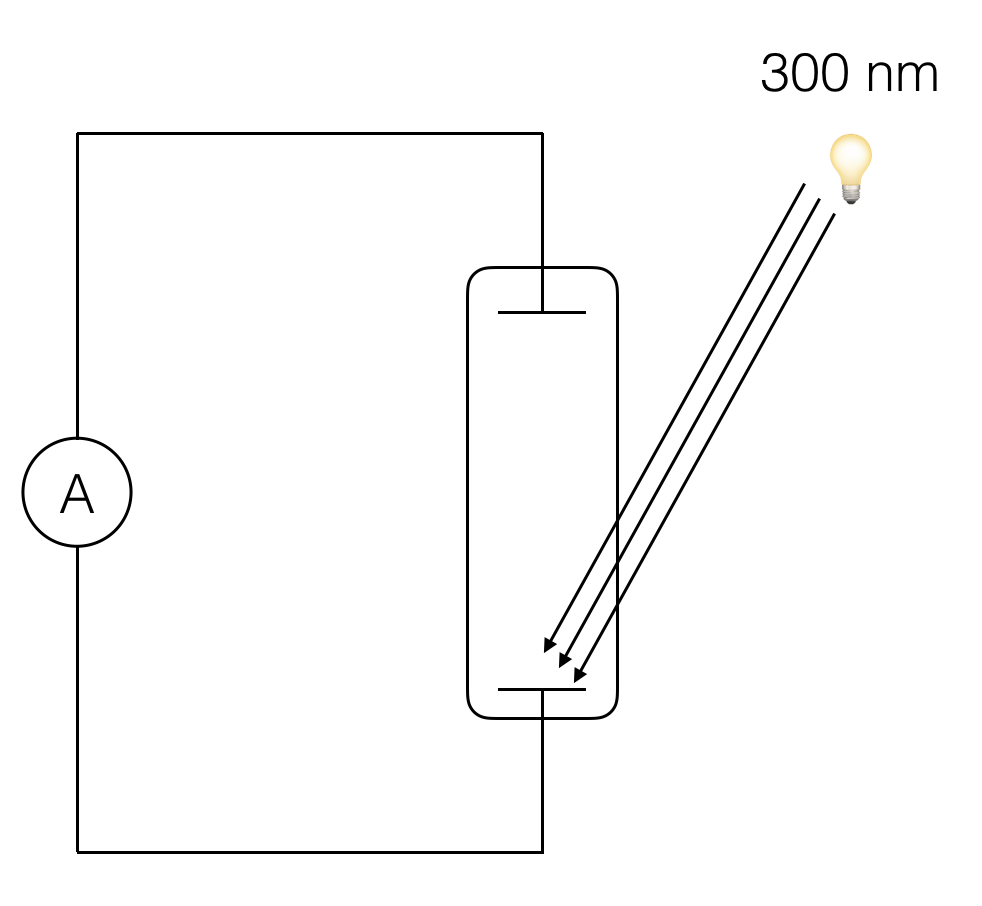
\includegraphics[width=0.45\textwidth]{../images/test2_300nm.png} 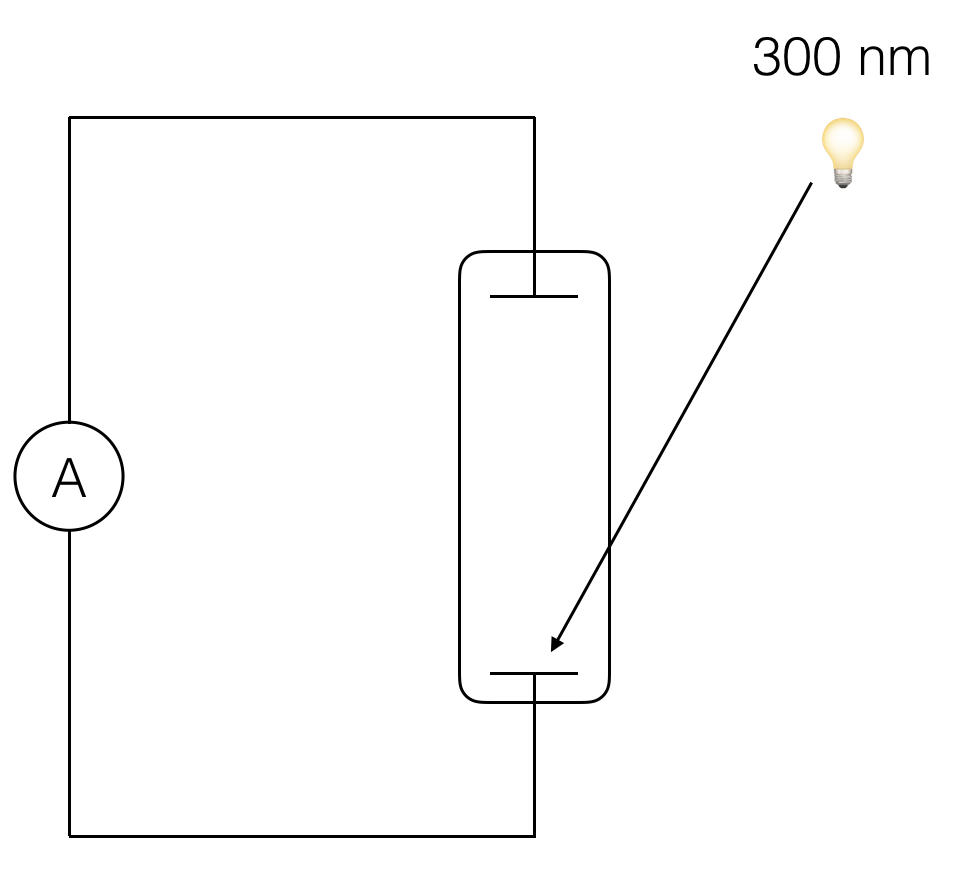
\includegraphics[width=0.45\textwidth]{../images/test2_300nm1.png}
\end{center}
	\begin{choices}
		\choice The two setups emit the same number of electrons, however the setup on the left emits electrons with greater energies.
		\choice The two setups emit the same number of electron, however the setup on the right emits electrons with greater energies.
		\choice The two setups emit electrons at the same energies, however the setup on the left emits more.
		\choice The two setups emit electrons at the same energies, however the setup on the right emits more.
		\choice The two setups emit the same number of electrons and at the same energies.
	\end{choices}
	\begin{TheSolution}
	\textbf{C.} Since light in both setups has the same wavelength, they transfer the same amount of energy to the electrons. However, since light on the left has a greater intensity it produces more photons and thus emits more electrons.
	\end{TheSolution}

\end{parts}
	
\bonusquestion \textbf{Creating Elements:} A nuclear physicist in a lab wishes to create oxygen. The graph below shows the binding energies for different elements and isotopes:
\noindent\begin{center}
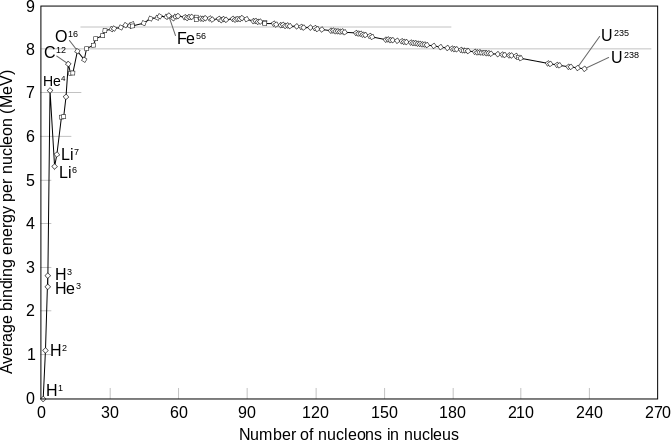
\includegraphics[width=0.9\textwidth]{../images/bindingEnergies.png}
\end{center}
\begin{parts}
	\part[2] She combines $^3He$ to create $^{16}O$. Overall, would this release or require energy?
		\begin{TheSolution}
			It would \textbf{release} energy. The binding energy for oxygen-16 is greater than that for helium-3, meaning that it would take more energy to break apart oxygen than helium. Conversely, it would release more energy to form oxygen than helium, meaning that to combine helium from oxygen it would release energy.
		\end{TheSolution}
	\part[2] She breaks apart $^{56}Fe$ to create $^{16}O$. Overall, would this release or require energy?
		\begin{TheSolution}
			It would \textbf{require} energy. The binding energy for iron-56 is greater than it is for oxygen-16.
		\end{TheSolution}
\end{parts}
\end{questions}



\end{document}